\documentclass[conference,a4paper]{IEEEtran}
\usepackage[T1]{fontenc}
\usepackage[utf8]{inputenc}
\usepackage[french]{babel}
\usepackage{amsmath,amssymb}
\usepackage{graphicx}
\usepackage{booktabs,tabularx}
\usepackage{microtype}
\usepackage{xurl}
\usepackage[hidelinks]{hyperref}
\graphicspath{{images/}}
\newcommand{\code}[1]{\texttt{\detokenize{#1}}}
\title{Adaptive Manipulation Lab :\protect\\
Conception et évaluation d'une chaîne d'apprentissage\protect\\
robotique par démonstrations et renforcement}
\author{\IEEEauthorblockN{Louis Lejaille}
\IEEEauthorblockA{Rapport technique R\&D --- 9 octobre 2026\\
\href{mailto:louis.lejaille@epitech.eu}{louis.lejaille@epitech.eu}}}
\begin{document}
\maketitle

\begin{abstract}
Adaptive Manipulation Lab associe démonstrations humaines et renforcement pour apprendre à un bras simulé dans MuJoCo à atteindre un cube. Trente démonstrations, soit 9\,067 transitions, servent à entraîner une politique par imitation (behavior cloning, BC), puis à initialiser Soft Actor-Critic (SAC). Les deux politiques figées sont évaluées sur 50 placements exclus de la collecte, de l'entraînement et de la sélection des checkpoints. Elles réussissent chacune 50 contacts sur 50. SAC réduit le temps moyen de contact de 5,96 à 2,01~s et augmente le retour moyen de 213,26 à 231,77. La comparaison appariée attribue ce gain à une réduction du nombre de décisions ; le critère de réussite reste le contact, sans exigence de prise stable. Le rapport décrit l'architecture, la collecte, le transfert et ses difficultés de stabilité. La robustesse à d'autres conditions physiques et l'extension à la saisie restent à évaluer.
\end{abstract}

\begin{IEEEkeywords}
robotique simulée, commande articulaire, MuJoCo, apprentissage par imitation, Soft Actor-Critic.
\end{IEEEkeywords}

\section{Introduction et objectifs du projet}
Le développement d'une politique de contrôle robotique repose sur la cohérence entre le modèle physique, l'espace de commande, les données d'apprentissage et les critères d'évaluation. Dans une tâche de manipulation, les contacts et les limites articulaires imposent des contraintes qui doivent être prises en compte dès la conception de l'environnement. Adaptive Manipulation Lab regroupe ces composants dans une plateforme expérimentale permettant la collecte humaine, l'apprentissage et l'évaluation sur une scène commune.

Le programme de développement vise l'approche, la saisie et le déplacement d'un objet. La première étape, nommée \code{reach}, consiste à établir un contact actif entre un cube et une géométrie de la pince. Le contact met fin à l'épisode. Ce périmètre permet d'étudier la commande articulaire et le transfert entre imitation et renforcement avant d'introduire les contraintes de maintien, de levage et de transport.

Les objectifs techniques sont de définir une interface commune au pilotage humain et aux politiques apprises, d'exploiter un ensemble limité de démonstrations pour initialiser le contrôle, puis de caractériser l'évolution de cette politique sous renforcement. L'instrumentation des entraînements et le versionnement des données permettent d'analyser les défaillances et de préserver les conditions de reproduction des expériences.

L'approche retenue associe trois moyens de contrôle. Le pilotage humain permet d'explorer la scène et de collecter des trajectoires. L'apprentissage par imitation (behavior cloning, BC) reproduit les actions sur les états observés. SAC poursuit l'optimisation par interaction avec la simulation. L'exploitation de démonstrations pour faciliter l'exploration en manipulation robotique a notamment été étudiée par Nair et al.~\cite{nair}. La méthode utilisée ici repose sur l'initialisation de l'Actor et l'import de transitions dans SAC ; elle diffère de leur approche fondée sur DDPG et HER. La figure~\ref{fig:pipeline} résume l'organisation des étapes.

\begin{figure*}[t]
\centering
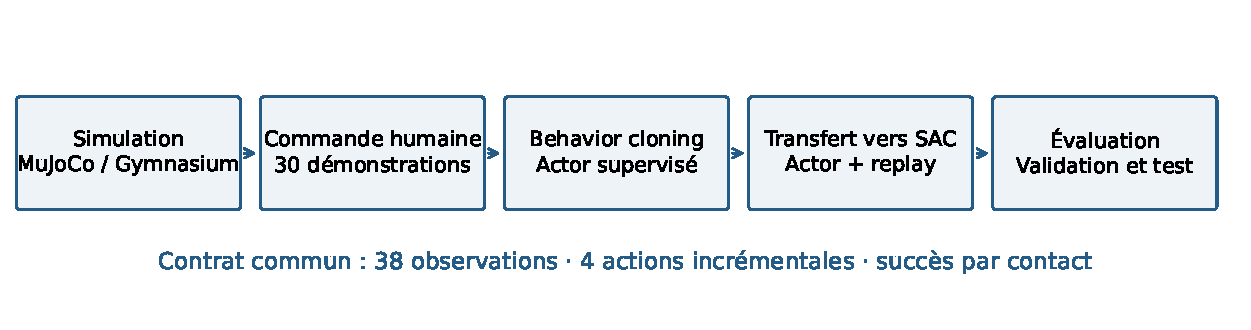
\includegraphics[width=\textwidth]{pipeline.pdf}
\caption{Chaîne d'apprentissage. La simulation, la collecte, le BC et SAC partagent le même contrat de commande. Les démonstrations de validation restent exclues du replay d'apprentissage. Une évaluation indépendante intervient après sélection et gel des modèles.}
\label{fig:pipeline}
\end{figure*}

\section{Périmètre et architecture logicielle}
\subsection{Organisation des composants}
Le projet est développé en Python avec NumPy, MuJoCo, Gymnasium et PyTorch. Pygame fournit l'accès à la manette ; pandas et matplotlib servent à l'analyse. SAC est implémenté directement dans PyTorch, sans dépendance à Stable-Baselines. Ce choix permet d'inspecter la cible de Bellman, les pertes et le transfert d'une politique BC dans l'Actor du SAC.

Le package \code{adaptive_manipulation} sépare les responsabilités. Le tableau~\ref{tab:architecture} décrit les principales couches. Les données expérimentales restent en dehors du package : \code{demonstrations/} conserve les sessions humaines, \code{runs/} les entraînements, \code{models/} la scène XML et \code{reports/} les audits.

\begin{table}[t]
\caption{Organisation du code exécutable}
\label{tab:architecture}
\centering\small
\begin{tabularx}{\columnwidth}{lX}
\toprule
Module & Responsabilité \\
\midrule
\code{core} & Configurations, chemins et versions de contrat. \\
\code{tasks} & Réussite par contact et calcul de récompense. \\
\code{simulation} & Scène MuJoCo, scénarios et adaptateur Gymnasium. \\
\code{interfaces} & Curseurs, manette et conversion des commandes. \\
\code{data} & Démonstrations, signatures, checkpoints et journaux. \\
\code{learning} & Actor, Critics, replay, BC et évaluation. \\
\code{workflows} & Collecte, entraînement, transfert et reprise. \\
\code{analysis} & Courbes issues des CSV. \\
\bottomrule
\end{tabularx}
\end{table}

La CLI expose \code{manual}, \code{record}, \code{inspect-demos}, \code{train-bc}, \code{train-sac}, \code{evaluate} et \code{plot}. Elle importe le workflow choisi à la demande : consulter l'aide générale ne charge pas les bibliothèques de simulation et n'ouvre pas de fenêtre. Cette séparation facilite l'utilisation du même dépôt pour l'interaction graphique et les entraînements sans affichage.

\subsection{Moteur de scénarios et interface d'apprentissage}
Le moteur \code{Environment} applique des consignes physiques absolues, avance MuJoCo et calcule les résultats des scénarios. Une session manuelle peut passer automatiquement au scénario suivant. L'adaptateur \code{ManipulationEnv} fournit l'interface Gymnasium attendue par les politiques : \code{reset}, \code{step}, observation vectorielle et actions normalisées.

Dans cet adaptateur, une fin d'épisode impose un appel explicite à \code{reset}. L'observation finale est conservée dans la transition terminale du replay, ce qui évite d'associer la dernière action d'un épisode à l'état initial du suivant. Le calcul de récompense est indépendant du réseau et partagé par la collecte et les entraînements.

\section{Conception de la simulation}
\subsection{Bras articulé et scène physique}
La scène de \code{models/robot_arm.xml} représente un bras fixé au sol. Il possède trois articulations rotatives : une rotation de base autour de l'axe vertical, une épaule et un coude autour d'axes horizontaux. Les segments principaux mesurent 0,50 et 0,40~m. Une pince symétrique comporte deux doigts coulissants, chacun limité à une course de 0 à 0,045~m. Les cinq actionneurs physiques reçoivent des consignes de position ; les deux actionneurs de pince utilisent une consigne commune.

Le cube a une arête de 0,08~m et une masse de 0,15~kg. Une articulation libre autorise sa translation et sa rotation. La zone initiale est une surface de 0,60~m de côté centrée en $(0{,}6,0)$ dans le plan horizontal. La figure~\ref{fig:simulation} présente l'état initial et l'état de contact final de la première démonstration enregistrée.

\begin{figure*}[t]
\centering
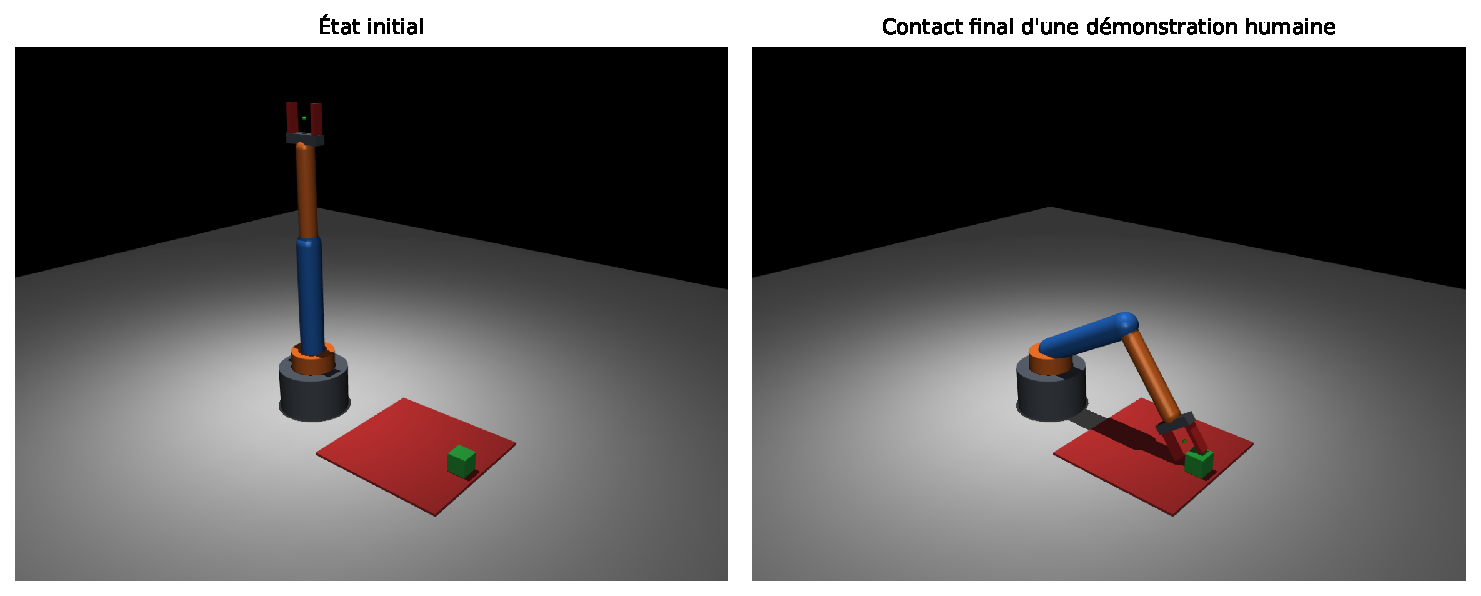
\includegraphics[width=.93\textwidth]{simulation.pdf}
\caption{Scène MuJoCo : état initial et contact final de la démonstration humaine 1. Le site central de la pince est représenté en vert ; le cube repose sur la zone de placement initial.}
\label{fig:simulation}
\end{figure*}

MuJoCo traite la dynamique articulée et les contraintes de contact~\cite{mujoco}. Le pas d'intégration du XML vaut 2~ms, sous gravité de $9{,}81~\mathrm{m\,s^{-2}}$, avec l'intégrateur \code{implicitfast}. Dans la configuration de référence, une décision avance au plus dix pas physiques, soit 20~ms et une fréquence nominale de décision de 50~Hz. Un contact ou une échéance peut interrompre ce groupe de pas avant sa fin.

\subsection{Placement reproductible de l'objet}
À chaque scénario, les positions, vitesses, forces et commandes sont remises à zéro ; la pince démarre ouverte. Le placement utilise un générateur pseudo-aléatoire initialisé par la seed du scénario. La marge tient compte de la demi-largeur du cube et de 5~mm supplémentaires : les coordonnées locales horizontales sont tirées dans $[-0{,}255;0{,}255]$~m. Dans le XML actuel, le centre du cube démarre donc dans
\begin{equation}
x\in[0{,}345;0{,}855],\qquad y\in[-0{,}255;0{,}255],
\end{equation}
avec $z=0{,}051$~m. Le moteur de placement prend également en compte la rotation de la zone. L'initialisation par seed permet de reproduire les placements lors des évaluations successives.

\subsection{Réussite et horizons de décision}
La réussite utilise un contact physique actif : la distance de contact MuJoCo doit être non positive et la contrainte correspondante active. La géométrie touchée doit appartenir à un doigt ou au support de pince. Un rapprochement du site central sans contact ne suffit pas, tandis qu'un contact avec le support est accepté.

L'épisode se termine au premier succès, à 20~s de simulation ou à 1\,000 décisions pour la configuration de référence. Ces deux budgets sont cohérents à 50~Hz, mais ils sont suivis séparément. Un contact survenant après l'échéance ne compte pas comme réussite. En apprentissage et en évaluation, l'horizon suit le temps physique MuJoCo ; l'interface manuelle utilise une horloge réelle.

Les échéances et limites de décision appartiennent à la définition de la tâche. Elles sont enregistrées comme \code{terminated=True}, avec pénalité d'échec, et non comme une troncature externe. Le replay conserve néanmoins séparément \code{terminated} et \code{truncated} pour distinguer les deux situations.

\section{Contrat d'observation et de commande}
\subsection{Une observation de 38 valeurs}
La politique reçoit un vecteur de 38 valeurs réelles, détaillé dans le tableau~\ref{tab:observation}. Les positions et vitesses sont obtenues directement depuis le simulateur. L'environnement correspond ainsi à un contrôle fondé sur l'état physique, sans module de perception visuelle.

\begin{table}[t]
\caption{Observation du contrat actuel ; indices Python semi-ouverts}
\label{tab:observation}
\centering\small
\begin{tabularx}{\columnwidth}{lcX}
\toprule
Indices & Taille & Contenu \\
\midrule
\code{0:12} & 12 & \code{qpos} : articulations, doigts, position et quaternion du cube. \\
\code{12:23} & 11 & \code{qvel} : vitesses généralisées. \\
\code{23:26} & 3 & Position du site central de pince. \\
\code{26:29} & 3 & Position du centre du cube. \\
\code{29:32} & 3 & Vecteur cube moins pince. \\
\code{32:36} & 4 & Consignes J1, J2, J3 et ouverture. \\
\code{36:38} & 2 & Fractions de temps et de décisions restantes. \\
\bottomrule
\end{tabularx}
\end{table}

Inclure les consignes est nécessaire parce que la commande est incrémentale : les positions physiques seules ne décrivent pas les cibles que les actionneurs poursuivent. Les deux budgets rendent l'approche de l'échéance observable. Les observations sont des copies, sans alias vers les tableaux internes de MuJoCo ; elles ne sont pas globalement normalisées par un prétraitement statistique.

\subsection{Quatre actions normalisées}
L'action $a_t\in[-1,1]^4$ contient trois demandes d'incrément articulaire et une demande d'incrément de pince. Si $u_t$ représente les consignes, la mise à jour est
\begin{equation}
u_{t+1}=\operatorname{clip}\bigl(u_t+a_t\odot v\,\Delta t,
u_{\min},u_{\max}\bigr),
\end{equation}
où $v$ regroupe les vitesses de consigne et $\odot$ désigne le produit composante par composante. La vitesse des articulations vaut $50^\circ/\mathrm{s}$ et celle des doigts $0{,}045~\mathrm{m/s}$. À 20~ms, une action maximale déplace la consigne de $1^\circ$ par articulation et de 0,9~mm pour chaque doigt. Ces valeurs bornent les incréments de consigne, pas la vitesse physique effectivement atteinte.

Les limites combinent les plages des articulations et des actionneurs. Une action demandée peut ainsi être écrêtée quand la cible atteint une borne. Les diagnostics distinguent l'action demandée, l'incrément effectif, la saturation de l'action et la présence de la cible à une limite. Cette distinction aide à interpréter une politique qui continue à commander dans une direction devenue inaccessible.

\section{Conception de la récompense}
La récompense $r_t$ désigne le signal reçu à chaque décision ; le retour $G=\sum_t r_t$ désigne leur somme non actualisée sur un épisode. Les tableaux et courbes de résultats présentent le retour, tandis que SAC optimise un objectif actualisé avec régularisation d'entropie. Le signal d'apprentissage combine un progrès géométrique, une variation de proximité, un coût de décision et une valeur terminale. Pour la distance $d_t$ entre le site de pince et le centre du cube, le potentiel de proximité est
\begin{equation}
\Phi(d)=20\exp\left[-\left(\frac{d}{0{,}30}\right)^2\right].
\end{equation}
La récompense implémentée à une décision est
\begin{align}
r_t={}&20(d_{t-1}-d_t)+\Phi(d_t)-\Phi(d_{t-1})\nonumber\\
&-0{,}1+b_t,\label{eq:reward}\\
b_t={}&\begin{cases}
200 & \text{si contact réussi},\\
-100 & \text{si échec terminal},\\
0 & \text{sinon}.
\end{cases}\nonumber
\end{align}
Les composantes sont calculées une fois par décision, y compris sur la dernière transition. Le contact est détecté indépendamment de la distance utilisée pour le shaping.

L'utilisation de variations signées évite qu'une succession d'allers-retours à la même distance accumule du progrès dans le retour non actualisé. Pour $N$ décisions, les termes géométriques se télescopent :
\begin{equation}
\sum_{t=1}^{N}r_t=20(d_0-d_N)+\Phi(d_N)-\Phi(d_0)
-0{,}1N+\sum_{t=1}^{N}b_t.
\end{equation}
À succès et états extrêmes identiques, le coût par décision favorise les trajectoires les plus courtes. Le télescopage concerne le retour non actualisé. L'objectif SAC utilise un facteur d'actualisation et une régularisation d'entropie ; le terme de proximité implémenté est une différence de potentiels non actualisée, distincte de $\gamma\Phi(s')-\Phi(s)$.

La distance finale décrit la position du site de pince par rapport au centre du cube, tandis que la réussite dépend des contacts entre géométries. La taille du cube et les dimensions de la pince expliquent qu'un épisode réussi conserve une distance finale non nulle.

\section{Collecte des démonstrations humaines}
\subsection{Pilotage et format de stockage}
Le bras peut être commandé par curseurs et par une DualSense. Les axes des sticks pilotent les trois articulations ; les boutons demandent l'ouverture, la fermeture ou le retour des consignes vers leur configuration initiale. Une zone morte de 0,15 limite la dérive des sticks au repos, avec remise à l'échelle progressive au-delà de ce seuil.

La collecte convertit ces entrées dans les mêmes quatre actions incrémentales que celles produites par l'agent. Une demande de fermeture ou de remise à zéro devient une suite d'incréments bornés ; elle ne provoque pas de saut instantané de consigne. Le BC apprend ainsi un comportement exécutable à travers l'adaptateur commun.

Un fichier compressé \code{episode_XXXX.npz} conserve les observations, actions, récompenses, observations suivantes et deux indicateurs de fin. Il stocke aussi les distances, temps simulés, diagnostics d'action et composantes de récompense. Les métadonnées identifient l'épisode, la seed, le placement, le résultat et la signature de l'environnement. \code{session.json} rassemble l'état de la session. Les épisodes interrompus sont séparés des épisodes complets.

\subsection{Jeu de référence et séparation par épisode}
La session \code{gamepad_30} contient 30 épisodes réussis, sur les seeds 3\,000\,000 à 3\,000\,029. Elle totalise 9\,067 transitions. La durée simulée moyenne des démonstrations est de 6,03~s, mais elle varie selon le scénario et le pilotage. La figure~\ref{fig:demonstrations} montre les placements et le volume de chaque épisode ; la figure~\ref{fig:human} illustre quelques trajectoires d'approche.

\begin{figure*}[t]
\centering
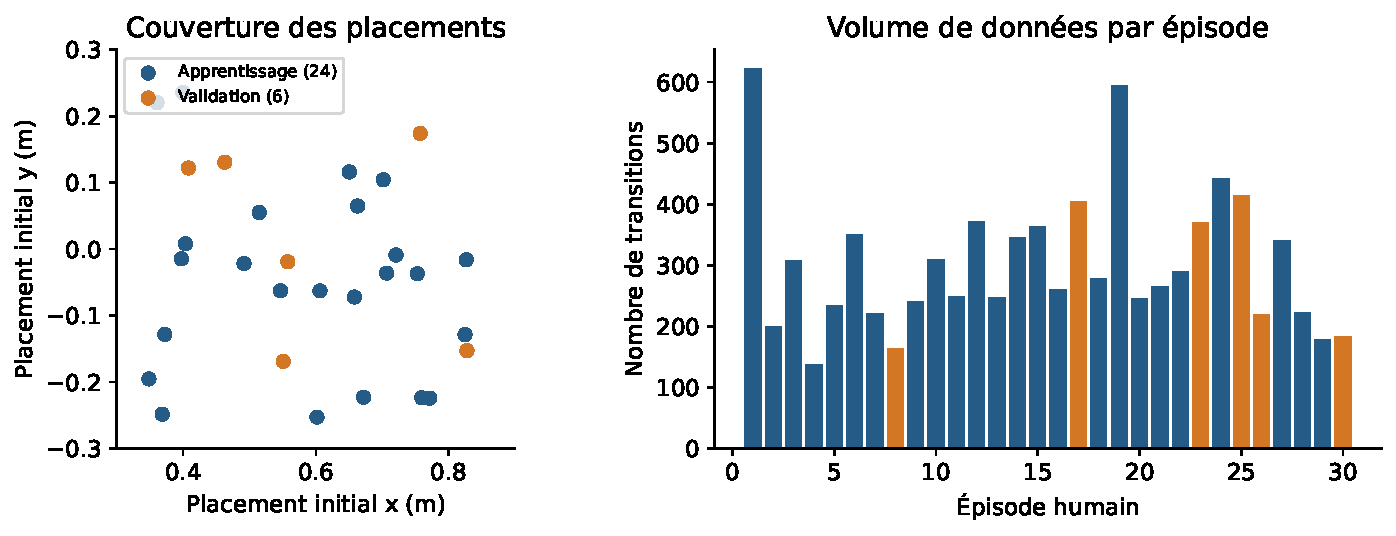
\includegraphics[width=.95\textwidth]{demonstrations.pdf}
\caption{Données humaines de référence. Le partage porte sur des épisodes entiers : 24 pour l'apprentissage et 6 pour la validation. Les couleurs identifient le même partage dans les deux panneaux.}
\label{fig:demonstrations}
\end{figure*}
\begin{figure}[t]
\centering
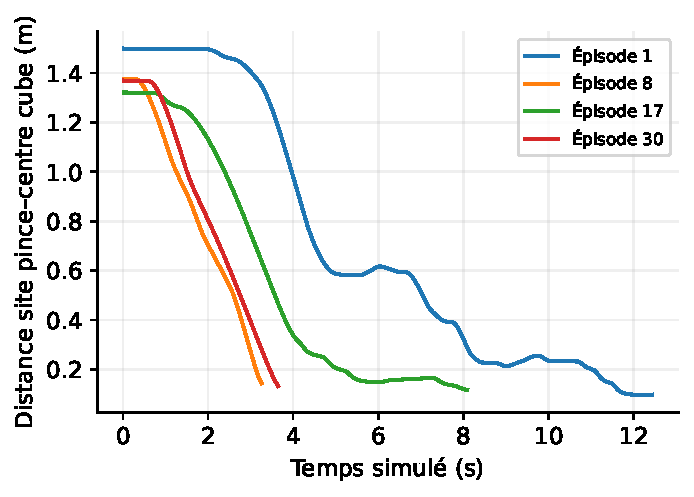
\includegraphics[width=\columnwidth]{human_distances.pdf}
\caption{Distances pince--cube dans quatre démonstrations enregistrées, choisies pour illustration. Chaque courbe s'arrête au contact physique ; la distance entre centres ne devient pas nécessairement nulle.}
\label{fig:human}
\end{figure}

Le split BC utilise la seed 42 et réserve 20\,\% des épisodes : 24 épisodes, soit 7\,312 transitions, pour l'apprentissage ; 6 épisodes, soit 1\,755 transitions, pour la validation. Les seeds réservées sont 3\,000\,007, 3\,000\,016, 3\,000\,022, 3\,000\,024, 3\,000\,025 et 3\,000\,029. Le partage par épisode réduit la fuite d'information qui résulterait d'un mélange aléatoire d'états voisins d'une même trajectoire.

La couverture du jeu de données est limitée à 30 trajectoires réussies. Les états successifs d'un même épisode sont corrélés et les comportements de récupération après échec sont peu représentés. Le volume de transitions doit donc être distingué du nombre de scénarios collectés.

\section{Apprentissage par imitation}
\subsection{Architecture et objectif supervisé}
Le BC réutilise l'Actor prévu pour SAC. Deux couches cachées de 256 neurones avec activations ReLU transforment l'observation. La sortie comporte huit valeurs, séparées en quatre moyennes gaussiennes et quatre logarithmes d'écart-type. L'action déterministe est $\tanh(\mu_\theta(s))$.

L'entraînement BC minimise l'erreur quadratique des actions humaines normalisées :
\begin{equation}
\mathcal{L}_{\mathrm{BC}}=\frac{1}{4M}\sum_{i=1}^{M}
\left\|\tanh(\mu_\theta(s_i))-a_i^{\mathrm{humain}}\right\|_2^2.
\end{equation}
La branche d'écart-type ne reçoit pas d'objectif d'imitation ; elle est initialisée pour produire un écart-type gaussien constant de 0,3. Ce paramètre fixe le niveau d'exploration initial lors du transfert vers SAC.

Adam utilise un taux de $3\times10^{-4}$ et des batches de 256 transitions. Le budget maximal est de 200 époques, avec une patience de 30 époques et un seuil d'amélioration de $10^{-6}$. La configuration enregistrée indique une exécution sur CUDA. Le checkpoint \code{best.pt} est choisi selon la MSE de validation, tandis que \code{latest.pt} conserve l'état le plus récent du BC.

\subsection{Convergence et exécution autonome}
Le meilleur checkpoint correspond à l'époque 16, avec une MSE de validation de 0,035287. L'entraînement s'arrête après 46 époques. La figure~\ref{fig:bc} présente les courbes globales et les erreurs par canal au checkpoint retenu. Le canal d'ouverture de pince présente une erreur nettement inférieure à celle des commandes articulaires. Cette mesure caractérise l'imitation des actions de la tâche d'approche.

\begin{figure*}[t]
\centering
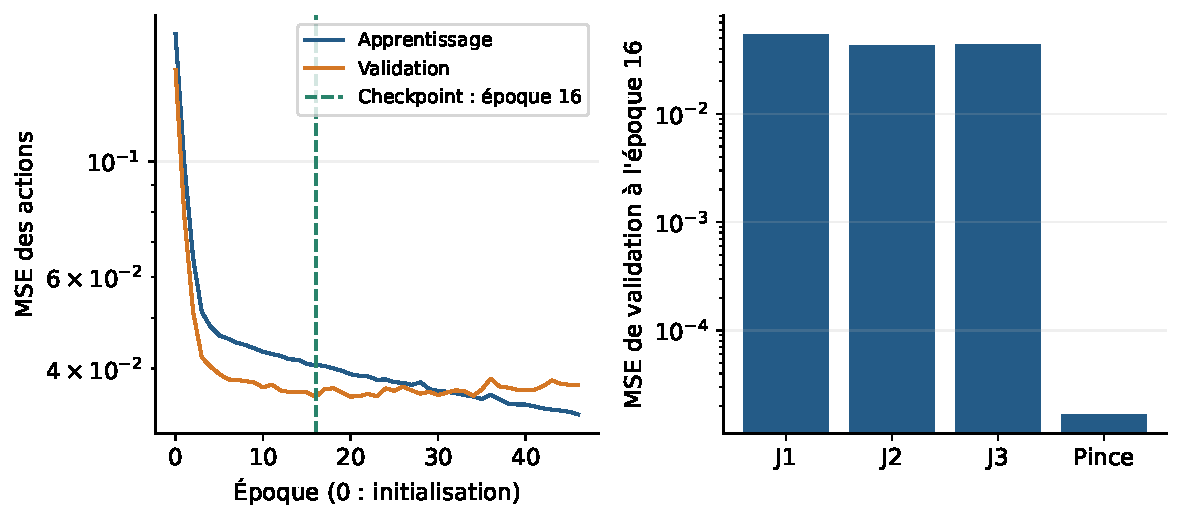
\includegraphics[width=.95\textwidth]{bc_learning.pdf}
\caption{BC : MSE d'apprentissage et de validation, puis erreur par canal à l'époque retenue. Les axes verticaux sont logarithmiques. L'époque 0 correspond au réseau avant optimisation.}
\label{fig:bc}
\end{figure*}

Les six rollouts déterministes du meilleur Actor réussissent. Le retour moyen vaut 210,58, le temps simulé moyen de contact 6,70~s et la distance finale moyenne 0,0939~m. La figure~\ref{fig:bcrollout} montre la variabilité entre scénarios. La durée moyenne humaine de 6,03~s est calculée sur l'ensemble des 30 démonstrations, tandis que la durée BC est calculée sur les six scénarios réservés ; les deux moyennes portent sur des populations différentes.

\begin{figure*}[t]
\centering
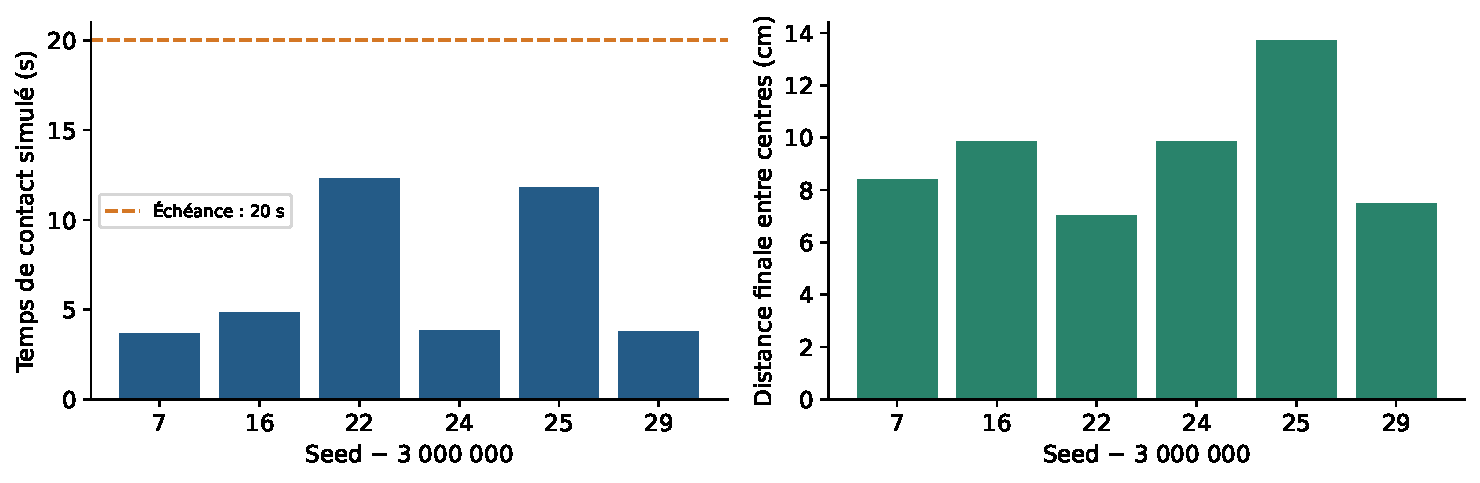
\includegraphics[width=.95\textwidth]{bc_rollouts.pdf}
\caption{Exécution autonome du meilleur BC sur les six seeds de validation. Tous les épisodes se terminent par contact. Le temps est celui de la simulation, et la distance finale est mesurée entre le site de pince et le centre du cube.}
\label{fig:bcrollout}
\end{figure*}

La MSE mesure l'imitation sur la distribution d'états des démonstrations, tandis que les rollouts évaluent la distribution induite par la politique autonome. Cette distinction est centrale en apprentissage séquentiel~\cite{ross}. Le taux de réussite observé confirme l'exécution de la tâche sur les scénarios réservés. Ces scénarios intervenant également dans la sélection du checkpoint, la mesure relève de la validation du modèle.

\section{Renforcement et transfert du BC vers SAC}
\subsection{Implémentation de Soft Actor-Critic}
SAC est un algorithme hors politique qui combine l'estimation de valeur et une politique stochastique avec régularisation par l'entropie~\cite{sac}. Le replay permet de réutiliser les transitions collectées, y compris des démonstrations compatibles avec la tâche. L'implémentation comporte un Actor, deux Critics $Q_1,Q_2$ et deux Critics cibles.

Les Critics utilisent chacun un MLP à deux couches de 256 neurones. Leur entrée concatène les 38 observations et les 4 actions. L'Actor échantillonne une gaussienne puis applique $\tanh$ ; le calcul de log-probabilité corrige cette transformation avec une expression numériquement stable. Les logarithmes d'écart-type sont bornés dans $[-20,2]$.

La cible de Bellman utilise le minimum des deux Critics cibles :
\begin{align}
y_t={}&r_t+\gamma(1-z_t)\bigl[
\min_{j\in\{1,2\}}\bar Q_j(s_{t+1},a')\nonumber\\
&\hspace{32mm}-\alpha\log\pi_\theta(a'\mid s_{t+1})\bigr],
\end{align}
où $z_t$ est l'indicateur \code{terminated} et $a'$ est échantillonnée par la politique. La perte de l'Actor est
\begin{equation}
\mathcal L_\pi=\mathbb E\left[
\alpha\log\pi_\theta(a\mid s)-\min_j Q_j(s,a)\right].
\end{equation}
La perte de l'Actor combine la log-probabilité des actions et leur valeur estimée ; son signe dépend de l'échelle des valeurs $Q$. Les Critics cibles suivent les réseaux en ligne par mise à jour douce.

\begin{table}[t]
\caption{Paramètres du run SAC initialisé depuis BC}
\label{tab:sacconfig}
\centering\small
\begin{tabular}{lr}
\toprule
Paramètre & Valeur \\
\midrule
Couches cachées Actor / Critics & $256,256$ \\
Taux Adam & $3\times10^{-4}$ \\
Actualisation $\gamma$ & 0,99 \\
Mise à jour cible $\tau$ & 0,005 \\
Température initiale $\alpha$ & 0,2 \\
Entropie cible & $-4$ \\
Batch / capacité du replay & 256 / 1\,000\,000 \\
Mises à jour par interaction & 1 \\
Préparation des Critics & 1\,000 mises à jour \\
Validation périodique & 10\,000 décisions \\
Budget configuré & 1\,000\,000 décisions \\
\bottomrule
\end{tabular}
\end{table}

La température est ajustée automatiquement~\cite{sacapplications}, avec une entropie cible de $-4$ pour quatre actions. Le tableau~\ref{tab:sacconfig} reprend les paramètres enregistrés. Le budget configuré est distinct de la portion effectivement présente dans les journaux.

\subsection{Transfert et préparation des Critics}
Le transfert charge les poids de l'Actor BC, puis vérifie le contrat d'environnement et l'architecture du réseau. Il importe uniquement les 7\,312 transitions de la partition d'apprentissage ; les 1\,755 transitions réservées ne sont pas versées au replay. Les empreintes des épisodes sont comparées à celles enregistrées au moment du BC.

Par défaut, les interactions utilisent les 24 seeds humaines d'apprentissage et la validation conserve les six seeds réservées. Les listes explicites de seeds prennent la priorité sur les intervalles génériques de configuration. Le transfert désactive la phase initiale d'actions uniformément aléatoires et rend les mises à jour disponibles dès le début.

Les 1\,000 premières mises à jour préparent les Critics, tandis que l'Actor et $\alpha$ restent fixes. Cette préparation se déroule pendant les interactions ; le robot utilise alors la politique BC déterministe. Elle ne correspond pas à un préentraînement exclusivement hors ligne. Après cette phase, les actions deviennent stochastiques et les mises à jour de l'Actor et de la température sont activées.

Une validation est enregistrée à la décision 0. Elle établit le niveau de départ et peut préserver la politique initiale dans le meilleur checkpoint si les étapes suivantes régressent. Le classement SAC privilégie le taux de réussite puis le retour moyen.

\section{Résultats et retour d'expérience}
\subsection{Audit d'un SAC initial sans démonstrations}
Une expérience historique, \code{sac_fixed_seed42}, utilisait un placement d'apprentissage unique, seed 42, et un ancien contrat de 36 observations. L'audit d'un checkpoint à 80\,000 décisions rapporte 80 épisodes, 79\,001 mises à jour et aucune réussite pendant ces épisodes. Le replay contenait 80\,000 transitions, aucune transition terminale et 80 fins enregistrées comme troncatures.

La distance moyenne dans ce replay était de 1,171~m ; seulement 0,1875\,\% des transitions étaient à moins de 30~cm, et aucune à moins de 10~cm. Le réseau disposait donc de très peu de données proches de l'objectif, sans exemple de succès. L'ancienne gestion des échéances autorisait en outre le bootstrap malgré une pénalité d'échec, sans exposer le budget restant dans l'observation.

Cet audit a conduit à trois modifications : ajout des budgets restants dans l'observation, traitement terminal des échecs et introduction de démonstrations d'approche. La modification simultanée du contrat de tâche et des données d'apprentissage limite l'analyse causale de l'amélioration. L'expérience historique sert à identifier les défaillances de la première configuration.

\subsection{Dynamique du SAC après initialisation BC}
La figure~\ref{fig:sac} révèle une évolution non monotone. Au départ, le SAC reprend les performances du BC : six réussites sur six et un retour moyen de 210,58. À 10\,000 décisions, la validation tombe à zéro réussite, avec un retour de $-165{,}73$. À 20\,000 décisions, les six contacts sont de nouveau réussis ; à 30\,000 décisions, la réussite est de cinq sur six. Les validations de 40\,000 à 90\,000 décisions donnent ensuite six sur six.

\begin{figure*}[t]
\centering
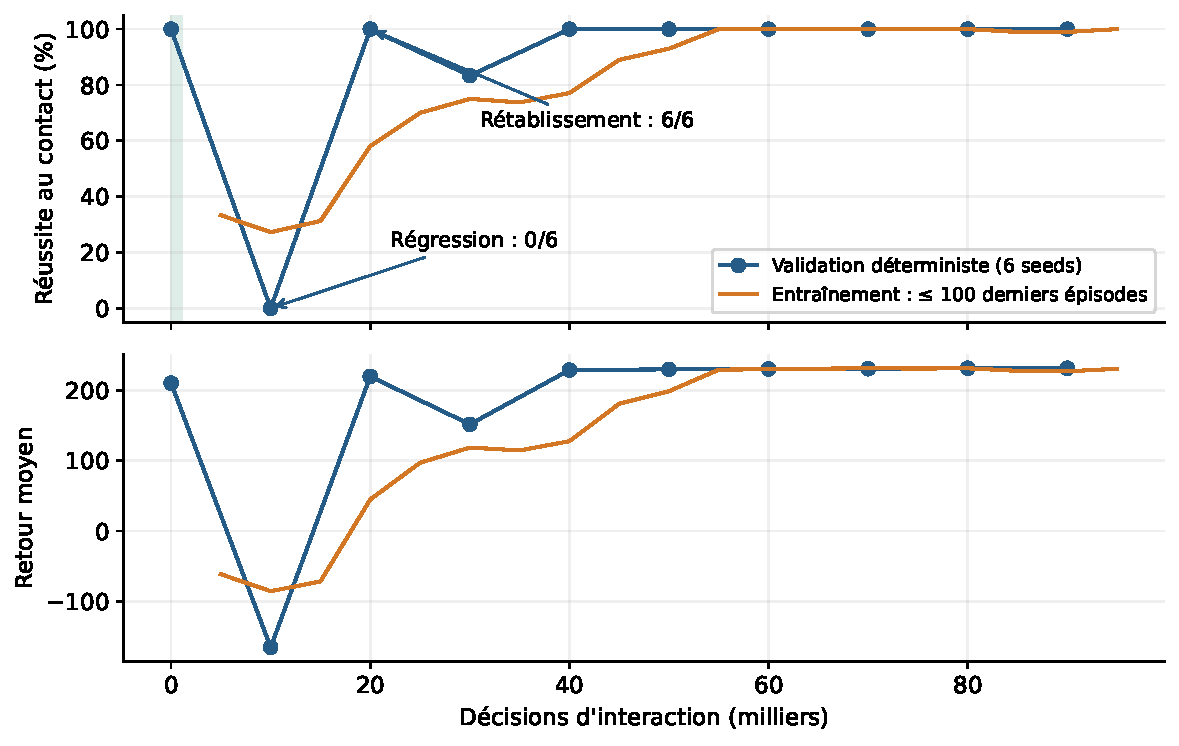
\includegraphics[width=.95\textwidth]{sac_progress.pdf}
\caption{SAC initialisé depuis BC : réussite et retour moyen. Les annotations identifient la régression à 10\,000 décisions (0/6), puis le rétablissement à 20\,000 décisions (6/6). La bande initiale représente les 1\,000 mises à jour de préparation des Critics. La validation déterministe porte sur six seeds ; l'entraînement utilise une fenêtre de 100 épisodes au maximum.}
\label{fig:sac}
\end{figure*}

La régression intervient après le passage à l'exploration stochastique et l'activation de l'optimisation de l'Actor. Ces changements exposent la politique à de nouvelles trajectoires et à des estimations de valeur encore en cours d'ajustement. Leur contribution respective reste à établir par ablation. Le niveau initial enregistré à la décision 0 fournit une référence pour le suivi du transfert et la sélection du meilleur checkpoint.

La dernière validation consignée correspond à 90\,000 décisions et 549 épisodes : réussite de 100\,\%, retour moyen de 231,72 et distance finale moyenne de 0,1266~m. Les journaux d'interaction se poursuivent jusqu'à l'épisode 634, terminé à la décision 98\,651 ; le dernier agrégat d'entraînement porte sur 95\,000 décisions. L'analyse de validation s'arrête à 90\,000 décisions, indépendamment du budget configuré d'un million de décisions.

Le tableau~\ref{tab:results} compare les deux checkpoints retenus sur les six placements de sélection, rejoués avec des actions déterministes sur CPU afin de disposer des temps individuels. Le checkpoint BC est celui de l'époque 16 ; le checkpoint SAC est celui de 90\,000 décisions. Le retour moyen augmente de 21,14 points et le temps moyen de contact passe de 6,70 à 2,07~s. La distance finale moyenne passe de 0,0939 à 0,1266~m, à taux de réussite identique. Les résultats rejoués reproduisent les agrégats historiques à l'arrondi près.

\begin{table}[t]
\caption{Validation sur les mêmes six seeds réservées}
\label{tab:results}
\centering\small
\begin{tabular}{lrr}
\toprule
Mesure & BC époque 16 & SAC à 90\,000 \\
\midrule
Réussite au contact & $6/6$ & $6/6$ \\
Retour moyen & 210,58 & 231,72 \\
Distance finale moyenne & 0,0939~m & 0,1266~m \\
Temps moyen de contact & 6,70~s & 2,07~s \\
Nombre moyen de décisions & 335,33 & 104,00 \\
\bottomrule
\end{tabular}
\end{table}
\begin{table}[t]
\caption{Comparaison appariée sur les six seeds de sélection}
\label{tab:pairedvalidation}
\centering\small
\begin{tabular}{rrrr}
\toprule
Seed$-3\,000\,000$ & BC (s) & SAC (s) & $\Delta G$ \\
\midrule
7 & 3.658 & 2.040 & 3.52 \\
16 & 4.840 & 2.544 & 10.29 \\
22 & 12.278 & 1.508 & 50.93 \\
24 & 3.850 & 2.432 & 5.78 \\
25 & 11.822 & 1.744 & 50.97 \\
29 & 3.752 & 2.154 & 5.35 \\
\bottomrule
\end{tabular}

\par\smallskip\footnotesize $\Delta G=G_{\mathrm{SAC}}-G_{\mathrm{BC}}$. Chaque paire réussit le contact.
\end{table}

\subsection{Évaluation indépendante sur 50 placements}
L'évaluation indépendante utilise les seeds 9\,000\,000 à 9\,000\,049. Leur absence des pools d'apprentissage et de validation, des métadonnées de collecte et des exports d'évaluation présents dans le dépôt a été vérifiée avant les essais. Le protocole fixe les deux checkpoints avant de produire les résultats ; aucune mise à jour ni nouvelle sélection de modèle n'est effectuée sur ces seeds. Les empreintes des checkpoints sont contrôlées avant et après les rollouts.

Chaque politique utilise le même environnement à 38 observations, les mêmes paramètres physiques et les mêmes placements initiaux. L'exécution sur CPU est déterministe. Les CSV conservent, pour chaque épisode, la seed, la réussite, le nombre de décisions, le retour, la durée simulée, la distance finale, la cause de terminaison et les composantes de récompense. Les six seeds de sélection sont évaluées séparément et restent exclues des agrégats indépendants.

Les deux politiques réussissent les 50 contacts. Aucun échec, timeout ou arrêt par limite de décisions n'est observé ; le journal d'échecs ne contient donc aucune entrée. Le tableau~\ref{tab:independent} présente les résultats, et la figure~\ref{fig:independent} leur comparaison par seed. Un intervalle de Wilson descriptif à 95\,\% pour 50 réussites sur 50 vaut $[92{,}9\,\%;100\,\%]$. Cette mesure concerne les placements de la même scène et des politiques fixes ; elle ne quantifie pas la variabilité entre entraînements ni la robustesse à une modification des conditions physiques.

\begin{table}[t]
\caption{Évaluation indépendante : mêmes 50 placements, politiques figées}
\label{tab:independent}
\centering\small
\begin{tabular}{lrr}
\toprule
Mesure & BC & BC + SAC \\
\midrule
Réussite au contact & $50/50$ & $50/50$ \\
Retour moyen & 213,26 & 231,77 \\
Temps moyen de contact & 5,96~s & 2,01~s \\
Nombre moyen de décisions & 298,36 & 101,14 \\
Distance finale moyenne & 0,1104~m & 0,1301~m \\
\bottomrule
\end{tabular}
\end{table}

\begin{figure*}[t]
\centering
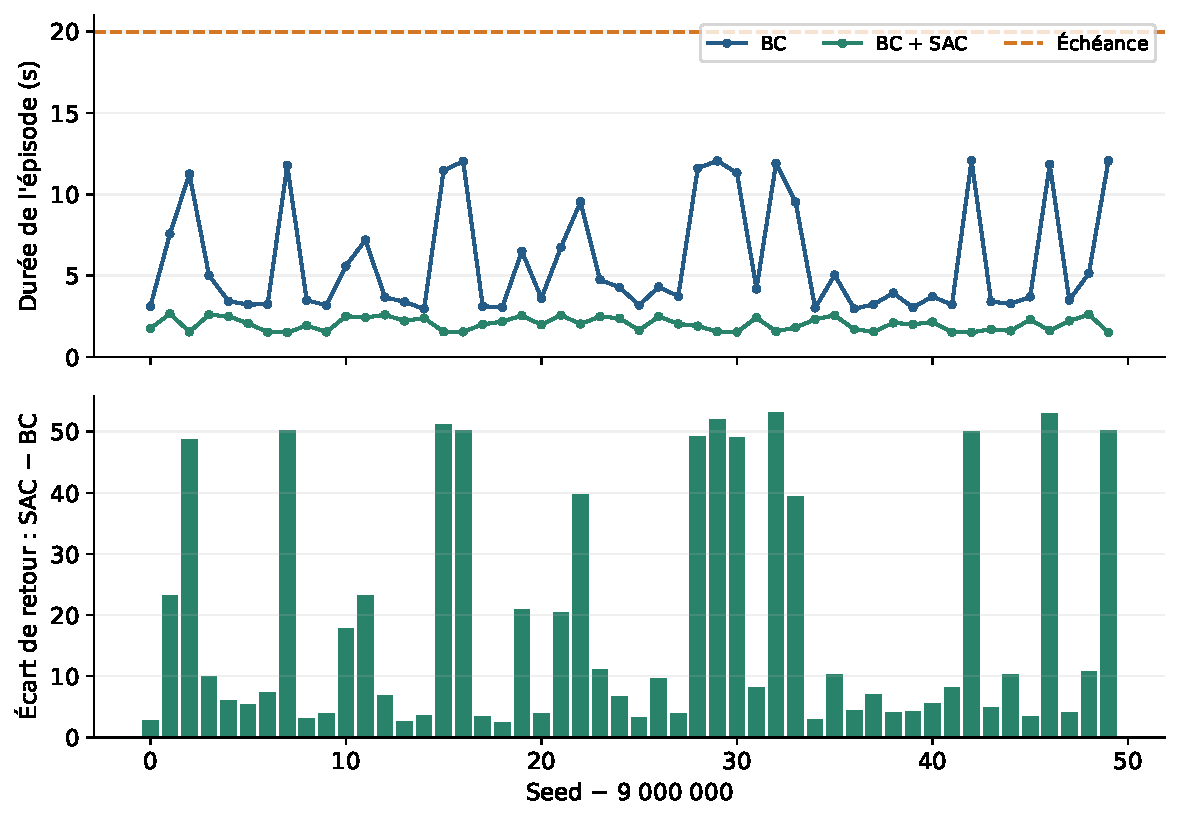
\includegraphics[width=.95\textwidth]{independent_comparison.pdf}
\caption{Évaluation indépendante appariée sur 50 seeds. En haut : temps simulé de contact des deux politiques, tous les épisodes étant réussis. En bas : différence de retour non actualisé, SAC moins BC. SAC atteint le contact plus vite sur chacune des 50 seeds.}
\label{fig:independent}
\end{figure*}

\subsection{Origine du gain de retour}
Pour une paire de rollouts partageant l'état initial et terminée par contact réussi, le bonus terminal est identique. En notant $G=\sum_t r_t$ le retour non actualisé, $N$ le nombre de décisions et $d_N$ la distance finale, l'écart entre SAC et BC s'écrit
\begin{align}
\Delta G={}&-0{,}1(N_{\mathrm{SAC}}-N_{\mathrm{BC}})\nonumber\\
&+20(d_{N,\mathrm{BC}}-d_{N,\mathrm{SAC}})\nonumber\\
&+\Phi(d_{N,\mathrm{SAC}})-\Phi(d_{N,\mathrm{BC}}).
\end{align}
Les composantes sont sommées pendant chaque rollout, ce qui permet de vérifier directement cette décomposition sans déduire le temps depuis le retour.

Sur les 50 placements, SAC économise en moyenne 197,22 décisions, soit 3,945~s de simulation. Le temps moyen diminue de 66,2\,\%, et les 50 différences appariées de durée sont favorables à SAC. La réduction du coût de décision apporte $+19{,}722$ points au retour moyen. Les changements de distance finale contribuent à hauteur de $-0{,}393$ pour le progrès et $-0{,}821$ pour la proximité, tandis que le bonus terminal reste identique. Le bilan est donc $+18{,}508$ points, égal à l'écart de retour mesuré. Sur les six seeds de sélection, le même calcul donne $+23{,}133-0{,}654-1{,}339=+21{,}140$ points. L'amélioration porte ainsi sur la rapidité du contact, et non sur le taux de réussite ou la distance finale.

\subsection{Diagnostics et interprétation des pertes}
Les journaux SAC distinguent les métriques d'épisode, les pertes, les Critics et les actions. Ils suivent notamment le désaccord entre Critics, les erreurs TD terminales et non terminales, l'entropie, l'écart-type de politique, les cibles en limite et l'erreur de suivi des actionneurs. La figure~\ref{fig:diagnostics} présente une sélection de ces signaux.

\begin{figure*}[t]
\centering
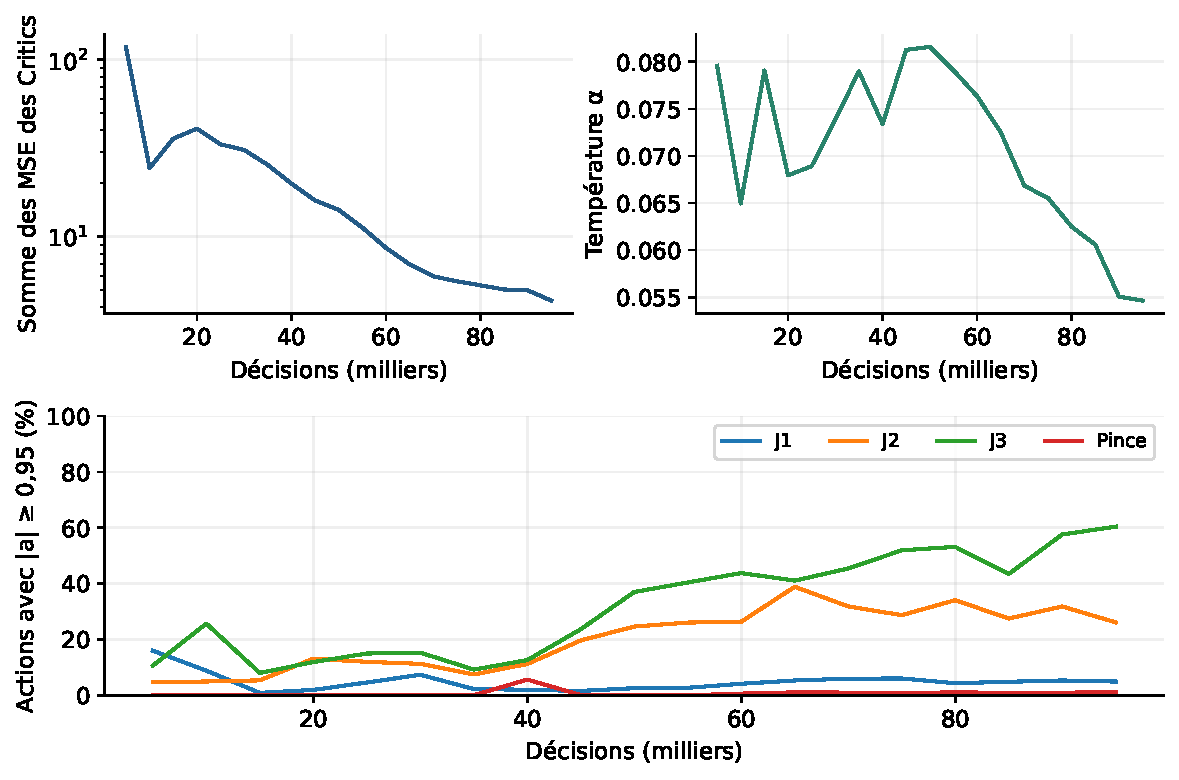
\includegraphics[width=\textwidth]{sac_diagnostics.pdf}
\caption{Diagnostics du SAC, agrégés par intervalles de journalisation : perte des Critics, température et proportion d'actions normalisées avec $|a|\geq0{,}95$. La saturation mesure l'amplitude demandée, indépendamment de la position des articulations.}
\label{fig:diagnostics}
\end{figure*}

À 95\,000 décisions, $\alpha$ vaut environ 0,0546 et la somme des pertes MSE des Critics 4,34. Sur la dernière fenêtre d'actions, le canal J3 présente 60,42\,\% d'actions avec $|a|\geq0{,}95$, ce qui indique un recours fréquent aux incréments proches de l'amplitude maximale. Les indicateurs d'écrêtage, de cible en limite et d'erreur de suivi complètent cette mesure pour caractériser la réponse physique.

L'analyse distingue trois niveaux : précision de l'estimation de valeur, comportement de commande et réussite de la tâche. Les pertes caractérisent les mises à jour des réseaux ; les diagnostics d'action décrivent les commandes appliquées ; les rollouts déterministes évaluent la politique résultante. Les métriques d'entraînement et de validation restent séparées en raison de leurs modes d'exploration et de leurs ensembles de seeds distincts.

\subsection{Traçabilité des évaluations complémentaires}
Un export complémentaire, \code{evaluation.csv}, contient dix contacts réussis sur les seeds 2\,000\,000 à 2\,000\,009. L'identité du checkpoint et sa configuration ne figurent pas dans les métadonnées de cet export. Les fichiers supplémentaires de \code{runs/evaluations/} présentent la même limitation de provenance. Ces mesures sont exclues de la comparaison BC/SAC.

L'évaluation indépendante présentée dans ce rapport associe au contraire les résultats à l'empreinte du checkpoint, à la signature physique, aux versions de contrat, à la liste des seeds et au mode d'action dans \code{protocol.json}. Ce format de provenance sera conservé pour les campagnes suivantes.

\section{Reproductibilité et fiabilité de la chaîne d'apprentissage}
\subsection{Signatures et sauvegardes}
Le contrat actuel utilise \code{observation_version=2} et \code{task_version=2}. Les signatures associent ces versions aux dimensions, à l'empreinte de la scène XML, aux incréments, aux limites et aux horizons. Le transfert BC vers SAC vérifie également l'architecture des réseaux et les empreintes des démonstrations importées. Les politiques du contrat historique à 36 observations sont incompatibles avec l'interface actuelle à 38 observations.

Un checkpoint BC contient l'Actor et la provenance du split. Un snapshot SAC complet conserve en plus les Critics et leurs cibles, les optimiseurs, la température, le replay, les générateurs aléatoires, l'état physique, les consignes et les compteurs. Cela permet une reprise au milieu d'un épisode. Le meilleur checkpoint SAC, plus léger, est destiné à l'évaluation ; une reprise complète utilise \code{latest.pt} ou un snapshot périodique.

Chaque nouvelle expérience utilise un répertoire de sortie distinct ; la reprise restaure un snapshot identifié. La configuration et les journaux restent ainsi associés à une exécution déterminée. La reproductibilité numérique dépend également du matériel et des versions de bibliothèques, en complément des seeds et états aléatoires sauvegardés.

\subsection{Vérification logicielle et traitement des données}
Les tests automatisés couvrent l'environnement, les démonstrations, les commandes, le BC, SAC, les diagnostics et le transfert. Ils vérifient les fins d'épisode, la cohérence des transitions, la compatibilité des contrats et les sauvegardes. La validation comportementale est réalisée séparément par les rollouts.

Les courbes d'apprentissage sont calculées à partir des journaux CSV, et les vues de simulation sont reconstruites depuis les états enregistrés dans les démonstrations. Les agrégats numériques et les empreintes des fichiers sources sont conservés avec les résultats. Les principaux artefacts expérimentaux sont répertoriés en annexe.

\section{Limites et prochaines étapes R\&D}
\subsection{Portée expérimentale actuelle}
La validité expérimentale des résultats est circonscrite à la tâche de contact, aux six scénarios de sélection et aux 50 placements indépendants de la même scène. Les principales limites concernent le critère de réussite, la diversité des données et les conditions physiques évaluées.

\textit{Critère de contact.} La terminaison au premier contact, y compris avec le support de pince, limite l'évaluation à l'approche. La qualité de fermeture, les efforts de préhension et le maintien de l'objet nécessitent des critères supplémentaires.

\textit{Étendue de l'évaluation.} Les six seeds interviennent dans la sélection des modèles et le suivi du développement. L'évaluation indépendante sur 50 nouvelles seeds complète cette validation, mais conserve la distribution de placement, le robot et les paramètres physiques de référence. Elle mesure une généralisation à de nouveaux placements dans cette distribution.

\textit{Variabilité entre entraînements.} Les expériences de référence ne comportent pas de répétitions à contrat identique avec plusieurs initialisations. La variabilité entre entraînements reste donc non quantifiée ; l'expérience historique utilise un contrat différent.

\textit{Couverture limitée des démonstrations.} Trente trajectoires réussies renseignent peu sur les états d'échec ou les comportements de récupération. Le BC peut rencontrer, en autonomie, des états éloignés de ceux de l'humain.

\textit{État physique directement observable.} Le contrôle utilise des poses et vitesses exactes du simulateur. La perception, le bruit de mesure et les délais d'un robot réel restent hors du périmètre évalué.

\textit{Diversité des conditions physiques.} Les essais concernent un seul bras, un cube et une scène. Le transfert sur matériel et la robustesse aux variations de masse, de géométrie ou de paramètres de contact restent à évaluer.

\subsection{Protocole d'ablation sous environnement commun}
La comparaison indépendante caractérise deux politiques issues d'une même chaîne BC vers SAC. Elle n'isole pas l'effet des démonstrations par rapport à un SAC entraîné depuis une initialisation aléatoire sous le contrat actuel. Les checkpoints SAC sans démonstrations disponibles utilisent 36 observations et ne constituent pas un témoin compatible. Une expérience d'ablation à trois configurations est donc prévue pour une campagne distincte (tableau~\ref{tab:ablation}).

\begin{table}[t]
\caption{Configurations de la campagne d'ablation envisagée}
\label{tab:ablation}
\centering\small
\begin{tabularx}{\columnwidth}{lX}
\toprule
Configuration & Question expérimentale \\
\midrule
SAC seul & Apprentissage depuis un Actor aléatoire, sans transitions humaines. \\
BC seul & Performance de l'imitation sans interaction d'optimisation supplémentaire. \\
BC + SAC & Effet du renforcement après initialisation par imitation et import des démonstrations. \\
\bottomrule
\end{tabularx}
\end{table}

Les trois configurations utiliseront le même XML, le contrat à 38 observations, la même récompense, les mêmes horizons et les mêmes pools de placements. Les branches SAC disposeront du même budget d'interactions et de mises à jour, en comptabilisant la préparation des Critics dans le budget BC + SAC. Le coût du préentraînement supervisé et la quantité de démonstrations seront rapportés séparément. Plusieurs seeds d'initialisation permettront d'estimer la variabilité entre entraînements. Les checkpoints seront sélectionnés sur la validation, puis évalués une seule fois sur un nouvel ensemble de test, distinct des 50 placements désormais utilisés dans ce rapport. Des ablations supplémentaires de la préparation des Critics et de l'import du replay humain permettront de distinguer les mécanismes du transfert.

\subsection{Extension à la saisie et au transport}
La tâche de saisie envisagée associera des contacts des deux doigts, une stabilité relative du cube et un maintien pendant une durée minimale. Le levage sera caractérisé par une hauteur et une durée de maintien ; le transport, par l'atteinte d'une pose cible et, selon le scénario, un relâchement contrôlé. Chaque étape disposera ainsi d'un critère de réussite distinct.

Les extensions de l'observation comprendront l'état des contacts, les vitesses relatives et la cible de déplacement. La récompense distinguera l'approche, l'établissement de la prise et sa stabilité. La collecte devra couvrir les séquences complètes de manipulation et les comportements de récupération. Ces évolutions seront associées à de nouvelles versions des contrats d'observation et de tâche.

L'extension nécessitera une sélection explicite de la tâche dans les workflows, actuellement associés à \code{reach}. L'intégration d'un second robot exigera une description de ses articulations, actionneurs, géométries de contact, sites et limites de commande. Les composants d'apprentissage pourront être réutilisés sous réserve de la compatibilité des dimensions et des contrats physiques.

\section{Conclusion}
Adaptive Manipulation Lab intègre la simulation, la collecte humaine, l'apprentissage par imitation et le renforcement dans une chaîne de contrôle commune. Le contrat de 38 observations et quatre actions incrémentales assure la continuité entre les démonstrations et les politiques autonomes. La gestion explicite des états terminaux, les signatures de compatibilité et les diagnostics constituent les principaux éléments de fiabilité de cette chaîne.

Les 30 démonstrations permettent d'obtenir une politique BC réussissant les six scénarios de sélection et les 50 placements indépendants. Le transfert vers SAC conserve ce taux de réussite et réduit le temps moyen de contact indépendant de 5,96 à 2,01~s, après une régression initiale en cours d'entraînement. La décomposition appariée attribue le gain de retour à la réduction du nombre de décisions. La campagne d'ablation sous contrat commun, la variabilité entre entraînements et l'extension à la saisie et au transport constituent les prochaines étapes.

\appendices
\section{Artefacts expérimentaux}
Les chemins suivants sont relatifs à la racine du dépôt. Ils identifient les données utilisées pour les résultats et les figures. Les répertoires d'entraînement regroupent leurs configurations, métriques et checkpoints.
\begin{table}[h]
\centering\small
\begin{tabularx}{\columnwidth}{lX}
\toprule
Artefact & Emplacement \\
\midrule
Scène physique & \path{models/robot_arm.xml} \\
Démonstrations & \path{demonstrations/gamepad_30/} \\
Apprentissage BC & \path{runs/bc_gamepad/} \\
Transfert et SAC & \path{runs/sac_from_bc/} \\
Audit historique & \path{reports/}\newline\path{sac_audit_metrics.json} \\
Évaluation appariée & \path{article/experiments/}\newline\path{heldout_50/} \\
\bottomrule
\end{tabularx}
\end{table}

\begin{thebibliography}{5}
\bibitem{mujoco} Google DeepMind, \emph{MuJoCo Documentation: Overview}. [En ligne]. Disponible : \url{https://mujoco.readthedocs.io/en/stable/overview.html}. Consulté le 9 octobre 2026.
\bibitem{sac} T. Haarnoja, A. Zhou, P. Abbeel et S. Levine, \emph{Soft Actor-Critic: Off-Policy Maximum Entropy Deep Reinforcement Learning with a Stochastic Actor}, 2018. \url{https://arxiv.org/abs/1801.01290}.
\bibitem{sacapplications} T. Haarnoja et al., \emph{Soft Actor-Critic Algorithms and Applications}, 2018, révisé en 2019. \url{https://arxiv.org/abs/1812.05905}.
\bibitem{ross} S. Ross, G. J. Gordon et J. A. Bagnell, \emph{A Reduction of Imitation Learning and Structured Prediction to No-Regret Online Learning}, AISTATS, 2011. \url{https://arxiv.org/abs/1011.0686}.
\bibitem{nair} A. Nair, B. McGrew, M. Andrychowicz, W. Zaremba et P. Abbeel, \emph{Overcoming Exploration in Reinforcement Learning with Demonstrations}, ICRA, 2018. \url{https://arxiv.org/abs/1709.10089}.
\end{thebibliography}
\end{document}
